\documentclass[main.tex]{subfiles}
\begin{document}

\section{Н. и д. условия асимптотической устойчивости линейных систем. Продолжение}

Напомним, если система устйчивая, то при записи в виде уравнения $\alpha(D)y =\beta(D)u$ должно выполняться условие: $Re(\lambda_i) < 0$, где $\lambda_i : \alpha(\lambda_i) = 0$

Разобрали случай различных корней.
Если же существуют кратные корни, в решении появится, в частности, слагаемое $ C_kt^k e^{\lambda_k t} $

Если вещественная часть меньше нуля, то экспонента <<задавит>> на бесконечности любой полином: $ y(t) \to 0 $ при $ t \to \infty $.
То есть н. и д. условие асимптотической устойчивости -- $ \boxed{Re \lambda < 0} $ (корни характеристического полинома лежат в левой полуплоскости).

Почему неравенство строгое?
При строгом устойчивость асимптотическая.
В МТУ нас интересует, как правило, асимптотическая устойчивость (а не устойчивость по Ляпунову).
Хотим, чтобы все колебания, неизбежно появляющиеся в  переходных процессов (например, флаттер в самолёте), затухали на бесконечности.

Напомним, $ \dot y - y = u + w \Rightarrow \lambda_1 = 1 > 0 \Rightarrow $ неустойчивая система.

\subsubsection{Важное следствие}

Напомним, мы нашли решение для возмущённого решения, для невозмущённого, вычли, получили однородное уравнение относительно $ \Delta y $:
\begin{align*}
    & \alpha(D) \Delta y = 0 \\
    & \Delta y = \sum c_i e^{\lambda_i t} \\
\end{align*}

Попробуем сразу найти общее решение: $ y(t) = y^+(t) + y^{++}(t) $, где $y^+$ -- общее решение однородного уравнения, $y^{++}$ -- частное решение неоднородного, которое определяется видом правой части.

Общее решение однородного уравнения содержит константы $ C_i $, которые определяются из начальных условий.

$$ y^+(t) = \sum C'_i e^{\lambda_i t} $$

Очевидно, $\lambda_i $ такие же, как в выражении для $ \Delta y $, но константы другие, т. к. берутся из начальных условий на $y$, а не на $\Delta y$.

Левая часть уравнения $ \alpha(D)y = \beta(D)u $ называют \emph{свободной} составляющей, правую -- \emph{вынужденной}.
Если $ Re \lambda_i < 0 $, экспоненты стремятся к нулю и решение $ y(t) \to y^{++}(t) $.

\textbf{Вывод:} если система устойчивая, решение при $ t \to \infty $ стремится к частному решению (к вынужденной составляющей, определяемой правой частью -- внешним воздействием).
Иногда это даже даётся как определение устойчивости.

Т. о. устойчивая система <<забывает>> начальные условия.
Пример: маятник с трением вне зависимости от начального угла и скорости в конце концов придёт к положению равновесия (покой).
Следовательно, можно начальные условия положить равными нулю, если нас интересует установившееся решение.

\subsection{Описание системы в пространстве состояний}

Напомним, в пространстве состояний три параметра: матрица $A$, вектор-столбец $B$ и строка $C$.

$$ \begin{cases}
\dot x = Ax + Bu \\
y = Cx
\end{cases} $$

Хотим выяснить: что отвечает за устойчивость?
Перейдём к преобразованию Лапласа:
\begin{align*}
    & \begin{cases}
        p \bar x = A \bar x + B \bar u \\
        \bar y = C \bar x
    \end{cases} \\
    & (pE - A) \bar x = B \bar u \Rightarrow \bar x = (pE-A)^{-1} B \bar u \Rightarrow \\
    & \bar y = C (pE-A)^{-1} \bar u \Rightarrow H(p) = C (pE-A)^{-1} \\
    & H(p) = \frac{\beta(p)}{\alpha(p)}, \thickspace \text{ порядок } \beta(p) < n, \text{ порядок } \alpha(p) = n
\end{align*}

Хотим найти корни $\alpha(p)$. $ A^{-1} = \frac{\tilde A}{|A|} \Rightarrow $

$$ \alpha(p) = |pE - A| = 0 $$

Это условие похоже на $ |A - \lambda E| = 0 $ (задача о нахождении собственных чисел матрицы $ A $).

Т. о. за устойчивость отвечает матрица $ A $ (её спектр): условие асимптотической устойчивости -- $ \boxed{ Re \lambda_A < 0 } $

\subsubsection{Устойчивость составных систем}

\begin{enumerate}[noitemsep]
	\item Последовательное соединение:
     $$ \rightarrow \boxed{\frac{\beta_1}{\alpha_1}} \rightarrow \boxed{\frac{\beta_2}{\alpha_2}} \rightarrow $$
     $\alpha = \alpha_1 \alpha_2 \Rightarrow H = H_1 H_2$ (передаточные функции перемножаются, и корни итогового характеристического полинома есть корни обоих), н. и д. условие устойчивости -- устойчивость обоих звеньев
	\item Параллельное соединение:

          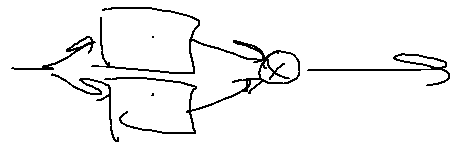
\includegraphics[width=.3\linewidth]{lec5/1parallel}

     $ H = H_1 + H_2 \Rightarrow $ это дробь, знаменатель будет таким же, как и в предыдущем пункте, и условие вновь сводится к устойчивости обоих звеньев.
	\item Система с обратной связью: принципиально иной случай.

    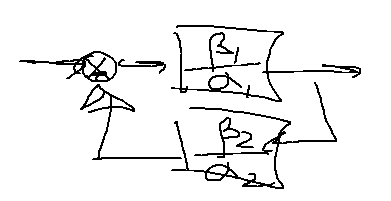
\includegraphics[width=.3\linewidth]{lec5/2backbind}

    $$ H = \frac{\frac{\beta_1}{\alpha_1}}{1 +  \frac{\beta_1 \beta_2}{\alpha_1 \alpha_2}} = \frac{\text{неважно что}}{\alpha_1 \alpha_2 + \beta_1 \beta_2} $$

    Пример.
    $$ \dot y - y = u + w $$
    Можно положить внешнее воздействие $ u = f(y) = -2y $, и система станет устойчивой: $ \dot y + y = \text{ неважно что } \Rightarrow \lambda_1 = -1 $.
\end{enumerate}

\subsection{ Критерии устойчивости линейных систем }
Рассмотрим устойчивую систему:
$$ \alpha(p) = 0, Re p_i < 0 $$

Даже для квадратного уравнения $ x^2 + bx + c = 0 $ можно найти такие такие $b,c$, что численные методы нахождения корней дадут сколь угодно далёкий от решения результат.

Научное сообщество разработало \emph{критерии} устойчивости линейных систем.
Они работают с коэффициентами полинома и значительно упрощают определение устойчивости.

У нас будут три алгебраических критерия и два частотных.

\subsubsection{Необходимое условие устойчивости Стодола}
Необходимое условие: позволяет браковать заведомо неустойчивые системы.

Стодола -- словацкий инженер (1890).
Следуя автору, запишем $\alpha(p) = a_0 p^n + ... + a_n $

Условие:
$$\boxed{a_i > 0} \text{ (точнее, коэффициенты одного знака)}$$

Доказательство.
$$ \alpha(p) = a_0 (p-p_1) \cdot ... \cdot (p - p_n); \alpha(p_i) = 0 $$

\begin{enumerate}[noitemsep]
	\item $ ] p_i \in \mathds{R} \to p_i = - \gamma_i^2 < 0 $ (необходимое условие устойчивости)
	$$ \alpha(p) = a_0(p+\gamma_1^2) \cdot .. \cdot (p + \gamma_n^2) $$

	Раскроем мысленно скобки: будет полный полином (все коэффициенты присутствуют), и их знак такой же, как знак $a_0$.
	\item $ ] p_i$  комплексно сопряжённые: $\begin{cases}
        p_1 = - \gamma_1^2 + j \delta_1 \\
        p_2 = - \gamma_1^2 - j \delta_1
    \end{cases} $
    $$ Re(p_i) < 0 \Rightarrow \alpha(p) = a_0(p + \gamma_1^2 - j \delta_1)(p + \gamma_1^2 + j \delta_1) \cdot ... = a_0 [(p + \gamma_1^2)^2 + \delta_1^2] \cdot .. $$


	Полный полином второго порядка; если раскроем скобки, все коэффициенты будут иметь знак $a_0$.
\end{enumerate}
Доказано.

Пример:

$ ] \alpha(p) = p^4 + 2 p^3 + 3p + 4 \Rightarrow $ неустойчивая система, т. к. нулевой коэффициент при $ p^2 $ и условие Стодола не выполняется.

Если же $ \alpha(p) = p^4 + 2 p^3 + 5 p^2 + 3p + 4 $, условие не работает и сказать о системе по критерию не получает.

\subsubsection{Н. и д. условия устойчивости Гурвица}

Гурвиц (1895 г): ему написал Стодола (не хватало математического образования).

Строим матрицу Гурвица:

$$ \Gamma_{n \times n} = \begin{pmatrix}
a_1 &  a_3 & a_5 & ... & 0 \\
a_0 &  a_2 & a_4 & ... & 0 \\
0   &  a_1 & a_3 & ... & 0 \\
... &&&& \\
0  &&& a_{n-2} & a_n
\end{pmatrix} $$

Критерий:

\begin{enumerate}[noitemsep]
	\item $ a_0 > 0 $
	\item $ \Delta_i > 0 $ (все главные миноры положительные)
\end{enumerate}

Пример:

$ ] n = 1 \Rightarrow \alpha(p) = a_0 p + a_1 \Rightarrow \text{ условие Гурвица: } p_1 = -\frac{a_1}{a_0} < 0 $

Совпадает с условием Стодола.

$ ] n = 2, \alpha = a_0 p^2 + a_1 p + a_2, p_{1,2} = \frac{-a_1 \pm \sqrt{a_1^2 - 4a_0 a_2}}{2a_0} $

\begin{enumerate}[noitemsep]
    \item Если дискриминант $ D < 0 $, то $ p_{1,2} = - \frac{a_1^2}{2 a_0^2} \pm j \frac{\sqrt{-D}}{2a} $.
    Т. о. условие Гурвица здесь -- $p_{1,2} < 0 $.
    \item $ D \ge 0 \Rightarrow p_1 = \frac{-a_1 - \sqrt D}{2 a_0} < 0 $

    $D = a_1^2 - x a_0 a_2, \thickspace a_0 > 0, a_1 > 0 \Rightarrow \sqrt D < a_1 \Rightarrow p_2 < 0 $ -- условие Гурвица.
\end{enumerate}



Вывод:
\begin{leftbar}
	Для систем I и II порядка необходимое условие совпадает с достаточным.
	Начиная с третьего порядка это не работает (необходимо дополнительное условие), и чем больше порядок, тем больше дополнительных условий.
\end{leftbar}

$ ] n = 3, \alpha = a_0 p^3 + a_1 p^2 + a_2 p + a_3 $

$$ \Gamma_{3\times3} = \begin{pmatrix}
a_1 & a_3 & 0 \\
a_0 & a_2 & 0 \\
0   & a_1 & a_3 \\
\end{pmatrix} $$

\begin{enumerate}[noitemsep]
	\item $ a_0 > 0 $
	\item $ Delta_1 = a_1 > 0 $
	\item $ Delta_2 = a_1 a_2 - a_0 a_3 \overset{a_0 > 0, a_3 > 0} > 0 $ -- этого условия нет в критерии Стодола!
	\item $ Delta_3 = a_3 \Delta_2 > 0 \Rightarrow a_3 > 0 $
\end{enumerate}

$$ \boxed{a_1 a_2 > a_0 a_3} \text{ -- дополнительное условие к критерию Стодола для систем III порядка} $$

Пример:
$$ p^3 + 2 p^2 + 3p + 5 \Rightarrow 2 \cdot 3 > 1 \cdot 5, \text{ система устойчива} $$

\subsubsection{Н. и д. условия Льенара-Шипара, 1914}

Пусть выполнены необходимые условия Стодола ($ a_i > 0 $).
Тогда можно упростить достаточное условие.

Составляем матрицу Гурвица $ \Gamma_{n \times n}  $.
Условия:

\begin{enumerate}[noitemsep]
	\item $ a_i > 0 $ (это условие Стодола)
	\item $ \Delta_{2k} > 0 $ ИЛИ $ \Delta_{2k-1} > 0 $ (можно проверять только чётные или нечётные миноры).
\end{enumerate}

То есть достаточно проверять вдвое меньше миноров.

Пример: если $ a_i > 0 $, мы посчитали миноры и оказалось, что все положительные, кроме одного, значит, мы ошиблись!

\subsubsection{Следящая система}

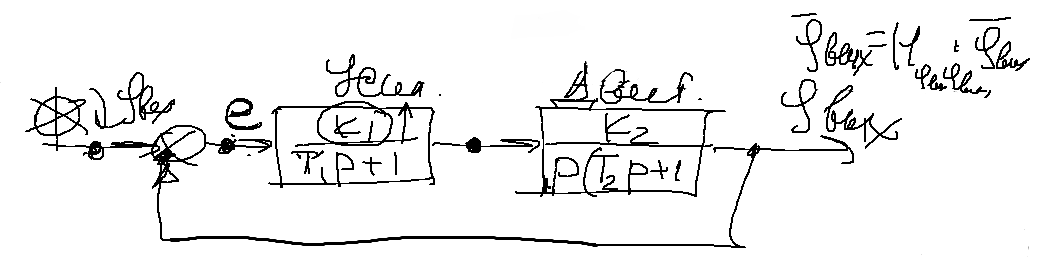
\includegraphics[width=.7\linewidth]{lec5/3control_system}

Рулевое колесо $ \Rightarrow $ сумматор $ \Rightarrow $ усилитель (обычно инерционное звено; $T_1$ мало, но всё же инерция) $ \Rightarrow $ двигатель.
На выходе двигателя -- угол; угол растёт линейно при постоянном входе $ \Rightarrow $ двигатель представляем как интегратор.

Обратная связь: выход мотора суммируется с $ \phi_\text{вх} $ так, что на вход усилителя поступает ошибка (отклонение реального угла поворота колёс от того, который задан рулевым колесом).
Цель: ошибка должна быть маленькой.

$ \bar e(p) = H_{\phi_{\text{вх}} e}(p) \cdot (\bar \phi_{\text{вх}}(p)) \xrightarrow[k \to \infty]{} 0 $, т. е. $ e(t) \to 0 $



(т. е. выход есть функция от входа на передаточную функцию; нам интересен не выход $\phi_{\text{вых}}$, а $e$ -- ошибка).

$$ H_{\phi_{\text{вх}} e}(p) = \frac{1}{1 + \frac{k}{p (T_1 p + 1)(T_2 p + 1)}} $$.
Значит, надо увеличить $k = k_1 \cdot k_2$, чтобы умньшать ошибку: $ \bar e(p) \xrightarrow[k \to \infty]{} 0 $

Почему мы не можем сделать ошибку бесконечно малой, уменьшая $ k_1 $ и $ k_2 $?

$$ H_{\phi_{\text{вх}} e}(p) = \frac{p (...)(...)}{T_1 T_2 p^3 + (T_1 + T_2) p^2 + k} $$

Система третьего порядка $ \Rightarrow $ для устойчивости недостаточно положительности всех коэффициентов $ \Rightarrow $ если потеряем устойчивость, ошибка будет стремиться к бесконечности.

Чтобы была устойчивость, нужно: $ T_1T_2 > 0, (T_1 + T_2) > 0, p + k > 0 $, а также $ (T_1 + T_2) > T_1 T_2 k $

$$ k < \frac{T_1 + T_2}{T_1 T_2} = \frac{1}{T_1} + \frac{1}{T_2} = k_{\text{критическое}} $$



\Large \textbf{Часть 2 лекции} \normalsize

Пример. Продолжение.

Пусть $\phi_{\text{вх}} = at \Rightarrow \bar \phi_{\text{вх}} = \frac{a}{p^2}$

$$ \bar e(p) = \frac{p(T_1 p+1)(T_2 p + 1)}{T_1 T_2 p^3 + (T_1 + T_2)p^2 + p + k} \cdot \frac{a}{p^2} $$

Хотим найти по предельной теореме ошибку в установившемся режиме:

$$ e_\infty = \lim\limits_{p \to 0} p \cdot \bar e(p) = \frac{a}{k} $$

Если $ k < k_{\text{критическое}} $,
$$ e_\infty > \frac{a}{k_{\text{крит}}} = a \frac{T_1 T_2}{ T_1 + T_2} $$

Ошибку невозможно сделать меньше величины $ e_{min} := a \frac{T_1 T_2}{ T_1 + T_2} $

\subsection{Частотные характеристики}

Частотные характеристики отражают поведение линейной динамической устойчивой системы при гармоническом воздействии.

Планеты движутся вокруг Солнца, электроны по орбитам, человек дышит...
Всё это колебания.

Пример:
\begin{enumerate}[noitemsep]
	\item Соотношение популяций волков и зайцев находится в динамическом равновесии (они находятся в противофазе и колеблются почти гармонически).
	\item Плавание: плотность тела такая, что мы не тонем, но уровень воды выше рта и носа, поэтому человек, не умеющий плавать, принимает вертикальное положение и пытается, работая руками и ногами, всё время держаться на поверхности.

	Но правильная стратегия -- привести себя в колебательное состояние: когда лицо над водой, делать вдох.
	Затраты на поддержание колебаний незначительные!
\end{enumerate}

Задача.

$$ \xrightarrow{u = u_0 \cos (\omega t)} \boxed{\frac{\beta (D)}{\alpha (D)}} \xrightarrow{y_\infty(t) = ?} $$

$y_\infty(t)$ -- установившаяся реакция

Система линейная, поэтому можно добавить мнимую часть (синус), чтобы легче было дифференцировать:

$ U = u_0 e^{j \omega t} = u_0 \cos (\omega t) + j \sin (\omega t) \to V(t) $

Линейная система $ \Rightarrow $ выход от вещественной части -- вещественная часть выхода, т. е. $ u_0 \cos (\omega t) \to Re(V(t)) $

$$ \alpha(D) Y = \beta(D) U $$

Устойчивая система, поэтому $ Y_\infty(t) = Y_{\text{частн}}(t) $

\begin{align*}
    \alpha(D)Y & = (\alpha_n D^n + ... + \alpha_1 D + \alpha_0) Y = \alpha_n (j \omega)^n Ce^{j \omega t} + ... + \alpha_1 (j\omega) C e^{j \omega t} + \alpha_0 Ce^{j \omega t} \\
    & = \alpha(j \omega) \cdot C e^{j \omega t} = \beta(D) \cdot u_0 e^{j\omega t} = \beta(j\omega) u_0 e^{j\omega t}
\end{align*}

А сейчас мы научимся мгновенно решать линейное дифференциальное уравнение любого (!) порядка, где в качестве возмущения есть синус или косинус.

$ e^{j \omega t} \ne 0 \Rightarrow $ сокращаем:

$$ \alpha(j \omega) = \beta(j \omega) $$

$$ C = \frac{\beta(j\omega)}{\alpha(j\omega)} u_0 \Rightarrow Y_{\infty}(t) = \frac{\beta(j \omega)}{\alpha(j \omega)} u_0 e^{j \omega t} $$

$ H(j \omega) = \frac{\beta(j \omega)}{\alpha(j \omega)} $ -- \emph{частотная передаточная функция} (ЧПФ): коэффициент, на который нужно умножить входной гармонический сигнал, чтобы получить выход.

Вытащим отсюда вещественную часть.
Частотная передаточная функция может быть представлена так: $ H(j\omega) = |H(j\omega)| e^{j \phi} $, $\phi$ -- аргумент:
$$ \phi = arg H(j \omega) = arctg \frac{Im(H)}{Re H}, \frac{-\pi}{2} \le \phi \le \frac{\pi}{2} $$
Т. о. $ Y_\infty(t) = |H(j\omega)| e^{j \phi} u_0 e^{j \omega t} = |H(j\omega)|u_0 e^{j(\omega t + \phi)} $

$$ \boxed{ y_\infty(t) = Re(Y_\infty(t)) = |H(j \omega)| u_0 \cos(\omega t + \phi) } $$

Выводы: если на входе гармонический сигнал, то на выходе гармонический сигнал той же частоты $ \omega $, амплитудой, увеличенной в $ |H(j \omega)| $ раз; сдвиг фазы $\phi$ (обычно $ \phi < 0 $).

\subsubsection{Виды частотных характеристик}

\begin{enumerate}[noitemsep]
    \item Амплитудно-частотная характеристика (резонансная кривая): зависимость амплитуды от частоты

    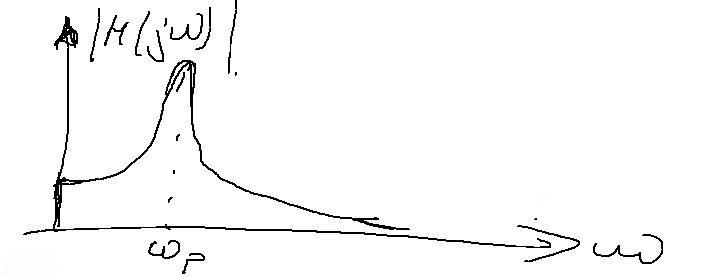
\includegraphics[width=.5\linewidth]{lec5/4afc}

    \item Фазо-частотная (фазово-частотная): зависимость сдвига фазы от частоты

    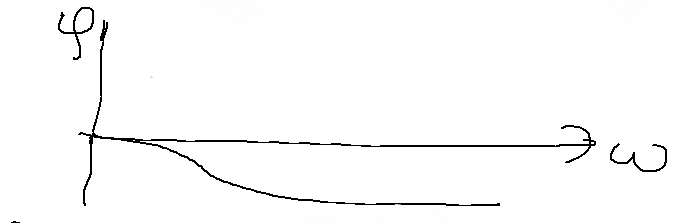
\includegraphics[width=.5\linewidth]{lec5/5apc}

    \item (Всеобъёмлющая характеристика) Амплитудно-фазовая характеристика (она же годограф ЧПФ -- частотной передаточной функции): траектория в осях $ Re (H(j\omega)) $, $ Im(H(j\omega)) $

    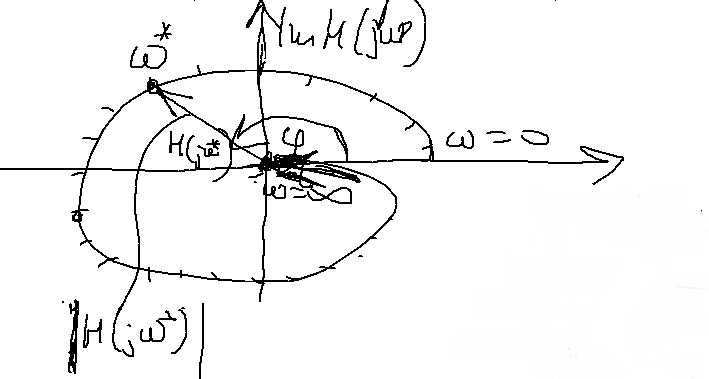
\includegraphics[width=.5\linewidth]{lec5/6apc}

    Часто это спирали, заканчивающиеся в нуле.
    Длина вектора из нуля в точку на АФК равна частоте $ \omega $, а угол поворота -- фазе $ \phi $.
\end{enumerate}

Примеры.

\begin{enumerate}[noitemsep]
	\item Интегрирующее звено:
    $$ H(p) = \frac{1}{p}, \thickspace H(j \omega) = \frac{1}{j \omega} = - \frac{j}{\omega} $$

    $|H(j \omega) = \frac{1}{\omega}|$ -- АЧХ.

    Фазо-частотная характеристика: фаза при всех частотах одинаковая и равна $ - \frac{1}{\omega} $

    Амплитудо-фазовая характеристика: смотрим, где лежат точки при всех частотах от $0$ до $ + \infty $.

    Движемся по мнимой оси вверх к нулю.

	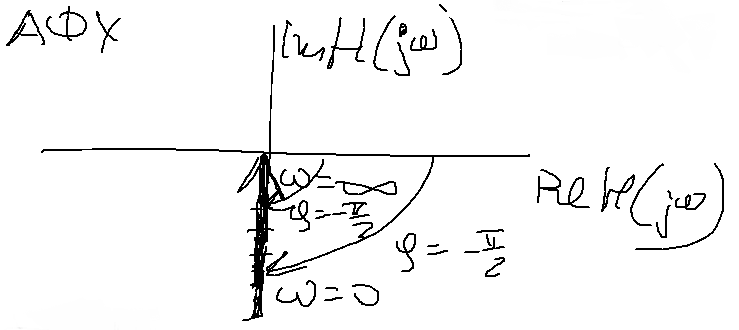
\includegraphics[width=.5\linewidth]{lec5/7apc}

	\begin{leftbar}
		Просьба в работах на осях писать $ Im(H(j\omega)), Re(H(j\omega))  $, а не просто $ Im, Re $.
        А то бешусь.
	\end{leftbar}

	\item Инерционное звено: резистор и конденсатор

	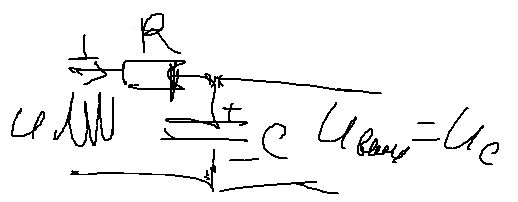
\includegraphics[width=.5\linewidth]{lec5/8integrator}

	$$ U_{\text{вых}} = U_C $$
	\begin{align*}
		& \frac{dq}{dt} = C\frac{du_C}{dt} \\
		& I = C \dot U_C \\
		& \begin{cases}
            \dot U = \dot U_R + \dot U_C \\
            U_R = IR
        \end{cases}
          \Rightarrow\\
        & \Rightarrow \dot U = \dot I R + \frac{I}{C} \\
		& \text{Иначе, } DU = DIR + \frac{I}{C} \Rightarrow I = \frac{DCU}{RCD + 1} \\
	\end{align*}

    размерность величины $ T = RC $ -- секунды, $ D $ -- $ \frac{1}{\text{сек}} $.

    $ U_C = I \cdot X_C,  X_C = \frac{1}{DC} \Rightarrow $

    $$ U_X = \frac{I}{DC} = \frac{U}{TD + 1} = H(D) U $$

    т. е. инерционное звено:

	$$ \boxed{H(p) = \frac{1}{Tp + 1}} $$

	Построим все частотные характеристики.

	$$ H(j\omega) = \frac{1}{1 + j \omega T} = \frac{1 - j \omega T}{1 + \omega^2 T^2} $$
	$$ |H(j \omega)| = \frac{1}{\sqrt{1 + \omega^2 T^2}} $$

	АЧХ:

	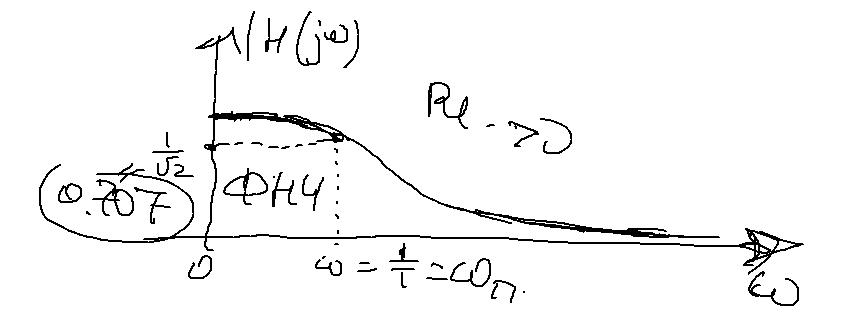
\includegraphics[width=.5\linewidth]{lec5/9afc}

	Считается, что, если $ \omega < \frac{1}{T} $, то сигнал (например, звук) проходит почти без искажений.
	Если выше, то это фильтр низких частот.

	ФЧХ:
	$$ \phi = arctg \frac{- \omega T}{1} = -arctg(\omega T) $$

	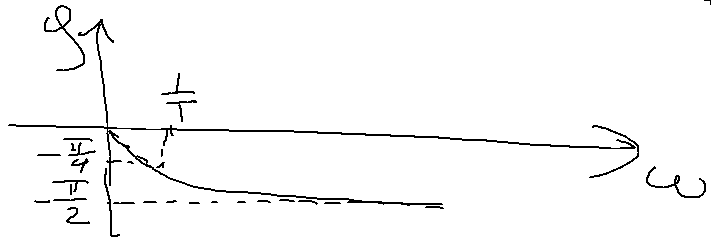
\includegraphics[width=.5\linewidth]{lec5/10apc}

	АФХ:

	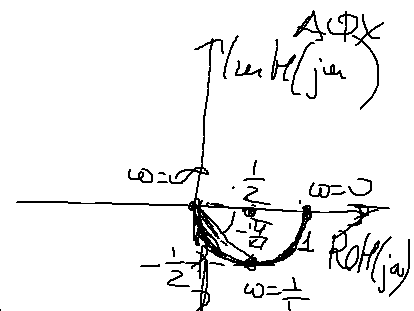
\includegraphics[width=.4\linewidth]{lec5/11pfc}

	$$ (Re H - \frac{1}{2})^2 + (Im H)^2 = \frac{1}{4} $$

\item Колебательная система (к примеру, стиральная машина):

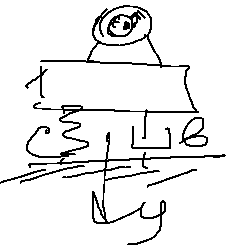
\includegraphics[width=.3\linewidth]{lec5/12washing}

$$ m \ddot y = -b \dot y - c y + F(t), \thickspace F(t) = F_0 cos(\omega t) $$
$$ H(p) = \frac{1}{p^2 + 2np + k^2}, \thickspace k^2 = \frac{c}{m}, 2n = \frac{b}{m} $$
$$ H(j \omega) = \frac{1}{(k^2 - \omega^2)^2 + 4 n^2 \omega^2} $$
$$ |H(j \omega)| = \frac{1}{\sqrt{(k^2-\omega^2)^2 + 4 n^2 \omega^2}} $$

АЧХ:

Если трение мало и частота равна собственной, будет пик.
Чем меньше $ n $, тем выше пик (вплоть до бесконечности).

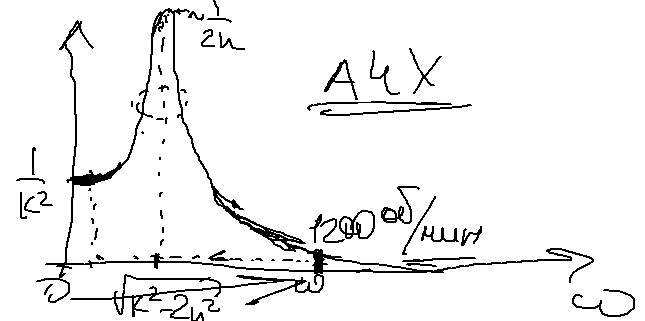
\includegraphics[width=.5\linewidth]{lec5/13afc}

Кому интересно, можно вывести дома: собственная частота $ = \sqrt{k^2 - 2n^2} $

АФХ:

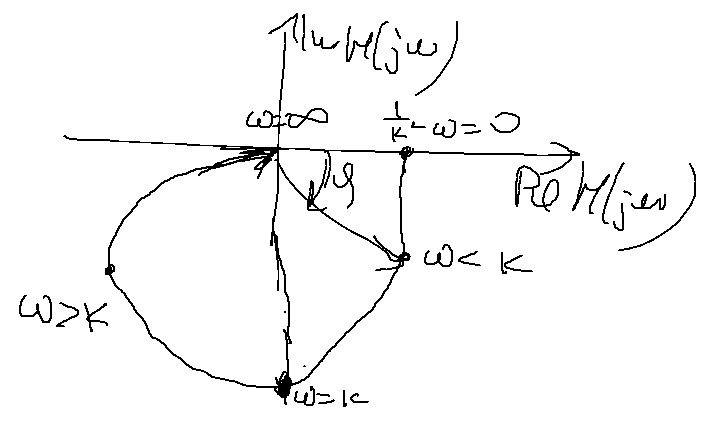
\includegraphics[width=.5\linewidth]{lec5/15pfc}

Когда $ \omega = k $, вечественная часть передаточной нулевая; $ \omega > k \Rightarrow $ отрицательная, $ < $ -- положительная.

При $ \omega \to \infty $ приходим, касаясь абсциссы, в ноль.

$$ \phi = \begin{cases}
arctg \frac{- 2n \omega}{k^2 - \omega^2}, \omega < k \\
arctg \frac{- 2n \omega}{k^2 - \omega^2} - \pi, \omega \ge k
\end{cases} $$

ФЧХ:

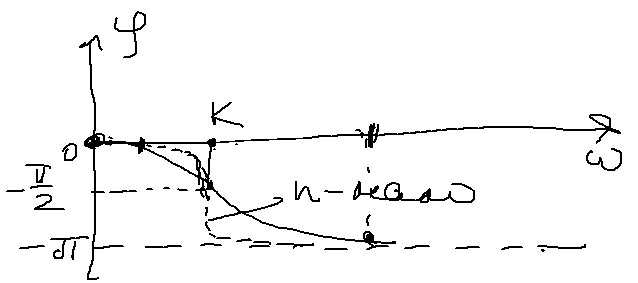
\includegraphics[width=.5\linewidth]{lec5/14apc}

Если $n$ мало, перегиб более крутой, в нуле -- функция Хевисайда.

Замечание: по АЧХ видно, что лучше всего работать на частоте больше, чем резонансная частота.
Стиральная машина быстро разгоняется, но при торможении (так называемый режим выбега) медленно проходит вниз по графику частот и может сильно трястись.

\item <<Раскидай>>: мячик на резинке. Диаметр примерно 4-5 мм.

Замечание: если подвесить раскидай как маятник и колебать с малой частотой, колебаться будет в такт.
Если частота велика $ \omega \approx 5 $ Гц, колебаться будет в противофазе.

В самом деле, раскидай, фактически -- грузик на пружинке.
Посмотрим на ФЧХ.

\item Светофор и машины: те, что стоят дальше от светофора в очереди, трогаются на красный.

\end{enumerate}

Оказывается, для определения устойчивости достаточно строить характеристики весьма приближённо.

\end{document}
